
\section{Conclusion}
%• Conclusions:
Throughout the design process multiple different setups very examined, see Section \ref{sec:platform}, by sustainable techniques such as scripting in Matlab, comparing hundreds of plots and establishing cost functions, determining the most optimal values. But this design phase also required some calculations of initial values from transform functions by solving differential equations, see Section \ref{sec:controllerstructure}, which are used as inputs to the controller. 

Then the connection between Matlab and the CompSOC was substantial in the assignment were the relations have to preserved in any calculation steps or examinations. Meaning that the modeling part only proves some fundamental components of the design but when system will be used, it is necessary to have tested the controller on hardware. In Figure \ref{fig:finalresult} the comparison between these two can be observed as well.

\begin{figure}[h]
	\begin{center}
		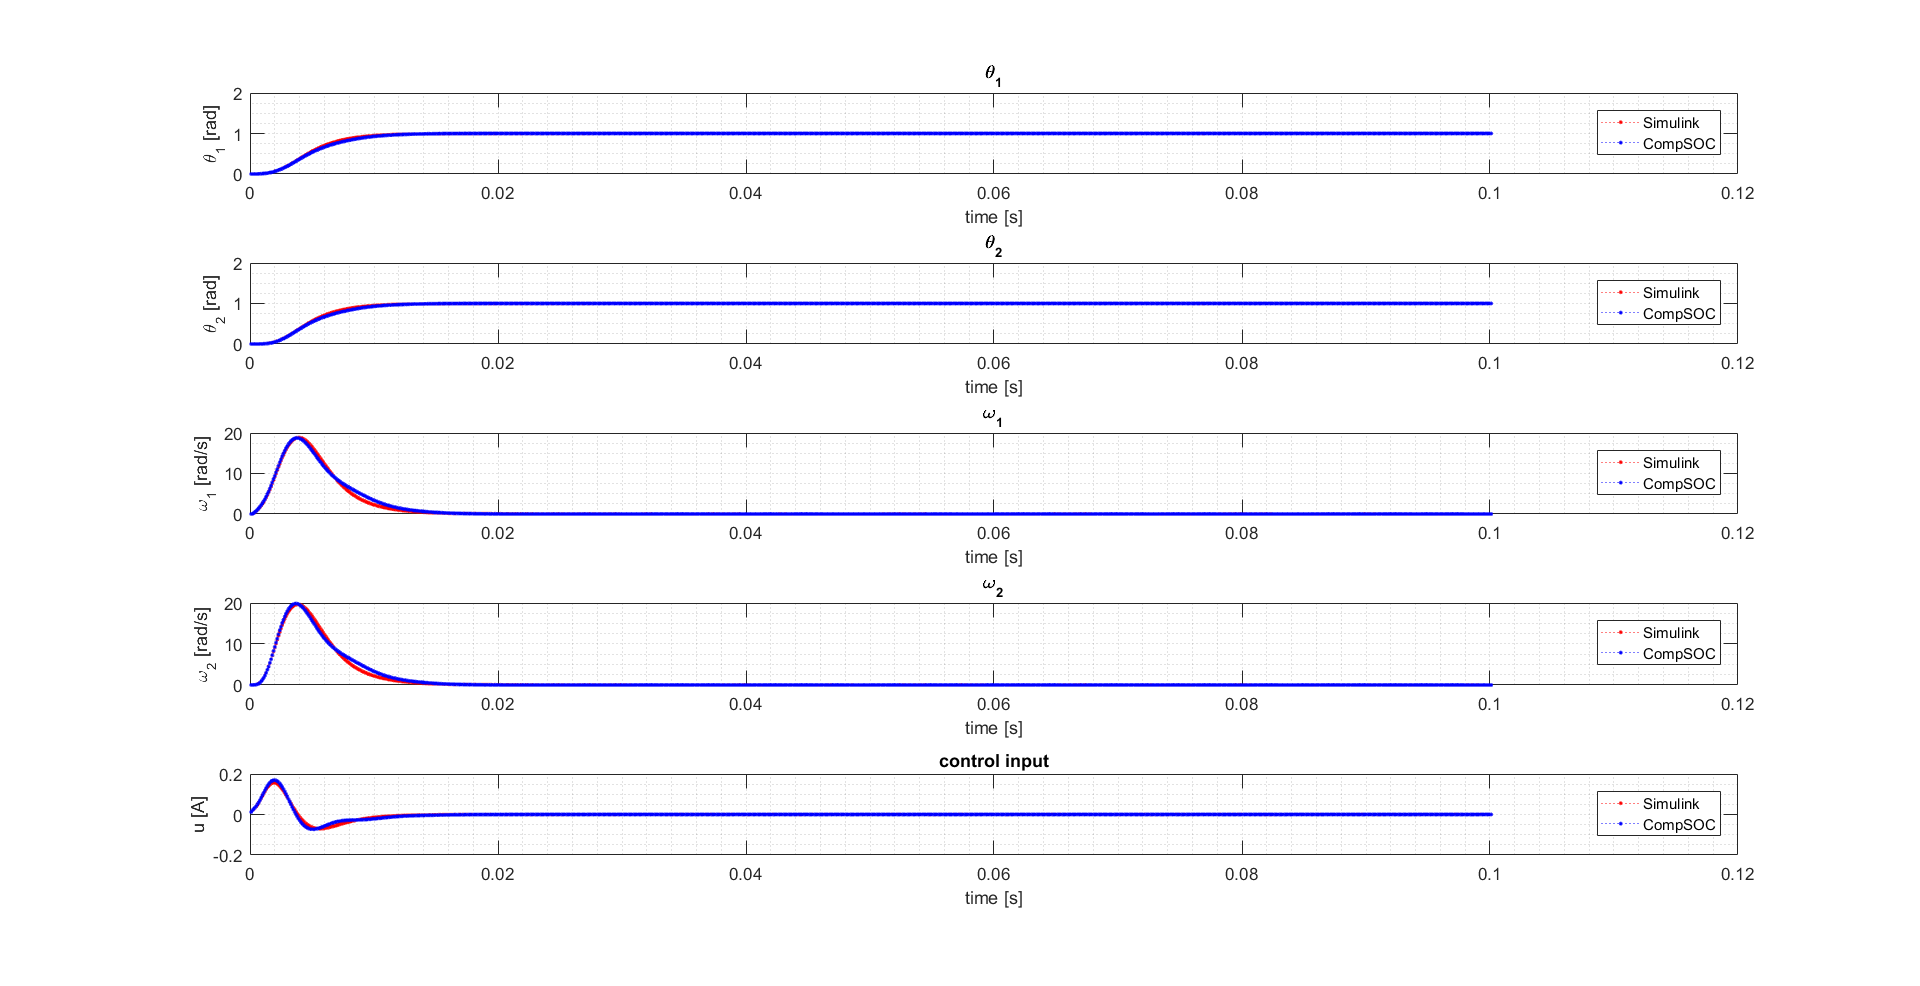
\includegraphics[width=\linewidth]{img/finalresult}
		\caption{Results comparison from Simulink and CompSOC.}
		\label{fig:finalresult}
	\end{center}
\end{figure}

All design requirements were met and an optimal solution was pursued with various optimization techniques. As requreste

\begin{enumerate}
	\item Modified CompSOC configuration file (sconfig.c)
	\item System states	and	control	input traces from the CompSOC platform (states.txt,	input.txt)
	\item Makefile used	to	specify	the	$USER\_TIMEOUT$	(makefile)
	\item MATLAB	control	design	script	$(stud\_control\_design\_a1.m)$
\end{enumerate}